\documentclass[11pt]{article}
\usepackage[top=1in, bottom=1in, left=1in, right=1in]{geometry}

\usepackage{amsmath}
\usepackage{amssymb}
\usepackage{graphicx}

\title{Quiz \#10, 11/17 \\ Math 156 (Calculus I), Fall 2023}
\date{}

\begin{document}

\maketitle

\thispagestyle{empty}

\vspace{-2cm}

Problem 1 is worth 5 points, and Problem 2 is worth 5 points, for a total of 10 points. Remember to \emph{show your work} on all problems!

\begin{enumerate}
\item Consider the curve $y=f(x)$ graphed below:
\vspace{-0.25cm}
\begin{center}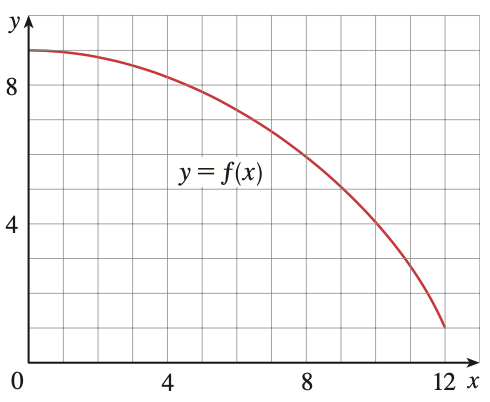
\includegraphics[width=1.75in]{quiz10.png}\end{center}
\vspace{-0.3cm}
Approximate the area under this curve from $x=0$ to $x=12$ by using three rectangles of equal width, where the heights are determined using the right endpoints of the three intervals.

\vspace{4cm}

\item Evaluate the following definite integrals by computing the relevant antiderivative and applying the Fundamental Theorem of Calculus.
\begin{enumerate}
\item $\int_{-1}^{1} x^2 + x \; dx$
\item $\int_{1}^{2} e^x \; dx$
\item $\int_{0}^{\pi} \sin(x) \; dx$
\end{enumerate}
\end{enumerate}

\end{document}